\documentclass[12pt]{article}
\usepackage{caption}
\usepackage{graphicx, subfig}
\usepackage{float}
\usepackage{mathptmx}
\usepackage{graphicx}
\usepackage{listings}
\usepackage{amsmath}
\usepackage{amssymb}
\usepackage{algorithm}
\usepackage{color}

\definecolor{dkgreen}{rgb}{0,0.6,0}
\definecolor{gray}{rgb}{0.5,0.5,0.5}
\definecolor{mauve}{rgb}{0.58,0,0.82}

\lstset{frame=tb,
  language=Python,
  aboveskip=3mm,
  belowskip=3mm,
  showstringspaces=false,
  columns=flexible,
  basicstyle={\small\ttfamily},
  numbers=none,
  numberstyle=\tiny\color{gray},
  keywordstyle=\color{blue},
  commentstyle=\color{dkgreen},
  stringstyle=\color{mauve},
  breaklines=true,
  breakatwhitespace=true,
  tabsize=3
}
\title{Exploration 1}
\author{Student Name: Fanjie Kong
\\
Student ID: 2462691 }

\begin{document}
\maketitle
\newpage
\textbf{Part 1 Classical HH	Model}
\\\\

1. Using	HodgkinHuxleyOriginal.py,	implement	the	classical	HH	model	as
described	in	the	handout	HodgkinHuxley.pdf.	In	the classical	model,	the	rest
potential	is	0.0	mV.
\\
 \begin{figure}[H]
  \centering
  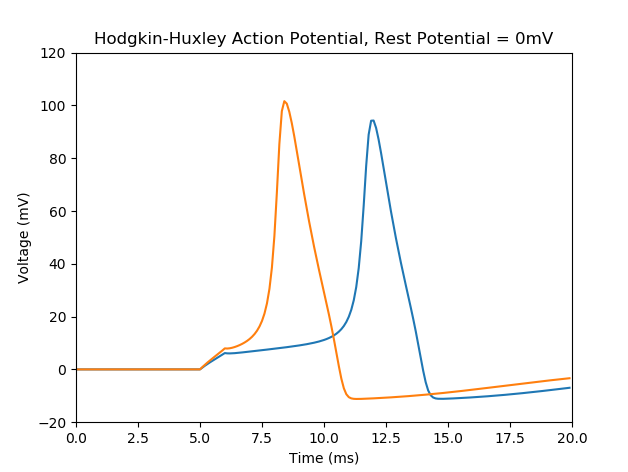
\includegraphics[width=.8\textwidth]{h1_p1.png} %1.png是图片文件的相对路径
  \label{img} %此处的label相当于一个图片的专属标志,目的是方便上下文的引用
  \caption{Result 1.1}
\end{figure}
\newpage

2. Change	the	model	so	the	rest	potential	is	-60.0	mV.	You	will	need	to	change	
the rate	constants	and	the	Nernst	potentials.	

\textbf{Answer:} 

\qquad
\\
 \begin{figure}[H]
  \centering
  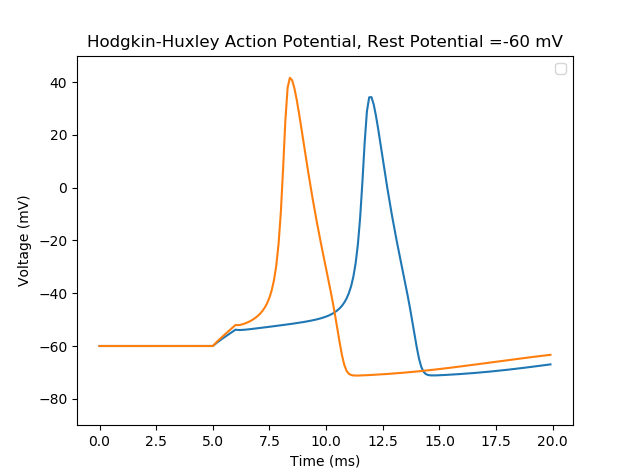
\includegraphics[width=.8\textwidth]{h1_p2.png} %1.png是图片文件的相对路径
  \label{img} %此处的label相当于一个图片的专属标志,目的是方便上下文的引用
  \caption{Result 1.2}
\end{figure}
\newpage

3. After	5msec,	apply	a	1	msec	pulse	and	determine	the	threshold	current	in	nA.
What	is	the	threshold.

\textbf{Answer:} 

\qquad The threshold is 1.5nA.

 \begin{figure}[H]
  \centering
  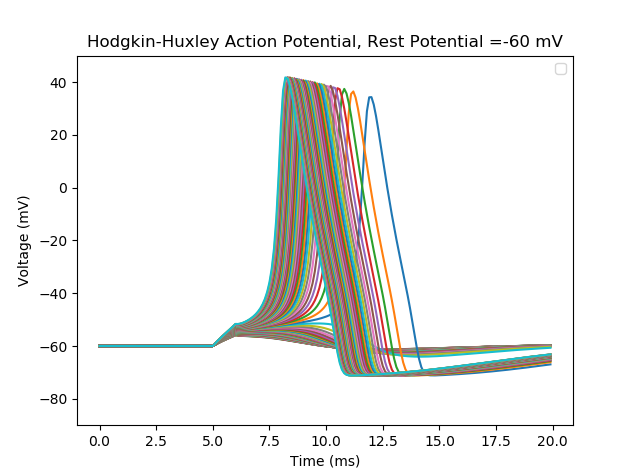
\includegraphics[width=.8\textwidth]{h1_p3.png} %1.png是图片文件的相对路径
  \label{img} %此处的label相当于一个图片的专属标志,目的是方便上下文的引用
  \caption{Result 1.3}
\end{figure}

\newpage

4. Apply	a	long	(2000	msec or	longer) pulse	with	amplitudes	ranging	from	0.0	
nA	to	7nA.	What	is the	firing	rate	as	a	function	of	current	amplitude?	Use	the	
code IF-HodgkinHuxleyOriginal-skel2.py	to	show	to	implement	100	neurons	
in	a group	and	apply	a	different	current	to	each	cell	from	0-99	with	the	
expression
$$group.I	=	'(7.0*nA	*	i)	/	num_neurons'$$
where	i	denotes	the	neuron	number.

\textbf{Answer:} 

\qquad The firing rate as a function of current amplitude is shown in the picture 

below.

 \begin{figure}[H]
  \centering
  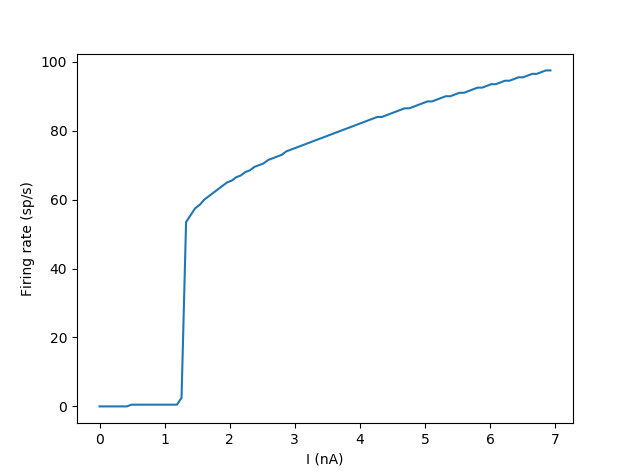
\includegraphics[width=.8\textwidth]{h1_p4.png} %1.png是图片文件的相对路径
  \label{img} %此处的label相当于一个图片的专属标志,目的是方便上下文的引用
  \caption{Result 1.4}
\end{figure}

\newpage
\textbf{Part 2 Connor Stevens Model}
\\

Modify	IF-ConnorsStevensOriginal-skel.py	to	become	the	Connor	Stevens	Model- see
handouts	connorstevens.pdf	and	ConnorStevensEqns.pdf.	This	will	involve	adding	
the variables	for	the	A	current.	The	A	current	is	given	in	terms	of	$a_{\infty}, \tau_{a}, b_{\infty}, \tau_{b}  $.	The
infinity	values	are	unitless	,	while	the	taus	have	units	of	ms.	Recall	that	the	
differential eqn	is	of	the	form

Reproduce	as	best	you	can	– Figure	6.1	in	connorstevens.pdf.	When	turning	off	the	A
current,	set	$gA=0$	and	$EL=-70mV$.	Explain	the	effect	of	the	A	current	on	the	firing	
rate using
$$group.I	=	'(7.0*nA	*	i)	/	num_neurons'$$
Use	the	approach	in	part	1	to	obtain	the	I	vs	Firing	rate	plot.
\\

\textbf{Answer:} 
\\

The A current constrains the rise time of the membrane potential between action potentials(Cited from Theoretical Neuroscience).

The A current let the firing rate much lower than the one without it. And it lets the firing rate rise continuously but not jump discontinuously.
\\

 \begin{figure}[H]
  \centering
  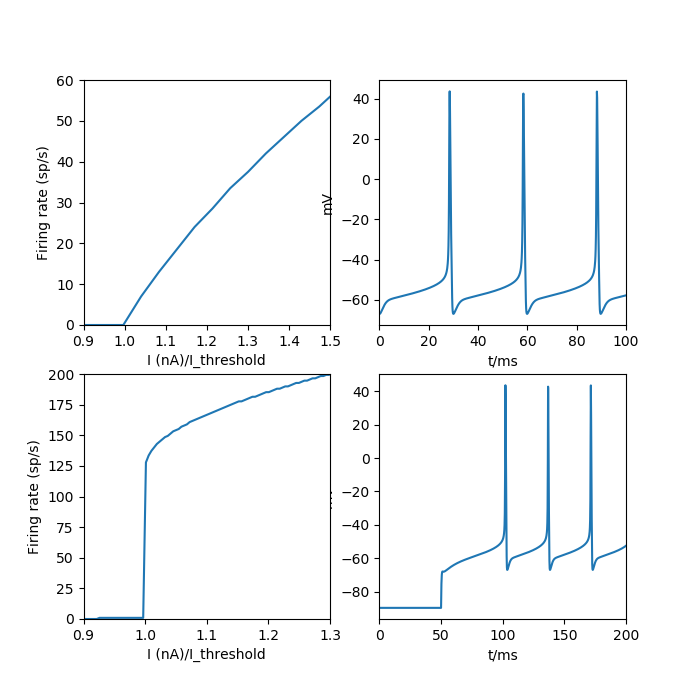
\includegraphics[width=1.2\textwidth]{h2_p1.png} %1.png是图片文件的相对路径
  \label{img} %此处的label相当于一个图片的专属标志,目的是方便上下文的引用
  \caption{Result 2.1}
\end{figure}

\newpage
\textbf{Part 3 Pyramidal Neuron}
\\

Using	IF-Pyramidal-skel.py,	reproduce	the	model	from the	Regular-spiking	(RS)	Ecell
in	the	paper	“Input-Dependent	Frequency	Modulation	of	Cortical Gamma	
Oscillations	Shapes	Spatial Synchronization	and	Enables	Phase	Coding”
(BiophysicalPyramidal.pdf	on	sakai).	Note	that	the	gating	variables	in	the	code	may	
have	different	letters.	You	can	adjust	as	you	wish.	
Use	the	approach	in	part	1	
$$group.I	=	'(7.0*nA	*	i)	/	num_neurons'$$
obtain	the	I	vs	Firing	rate	plot.
Explain	how	the	firing	rate	plot	compares	with	Hodgkin	Huxley	or	Connor	Stevens.
\\

\textbf{Answer:} 
\\

	H-H: The firing rate of Pyramidal model rises continuously from zero point with higher values. 
	
	Connor Stevens: The firing rate of Pyramidal model has much higher values than the firing rate of Connor Stevens model. And the rising rate(derivative) is increasing firstly, and then decreasing.
 \begin{figure}[H]
  \centering
  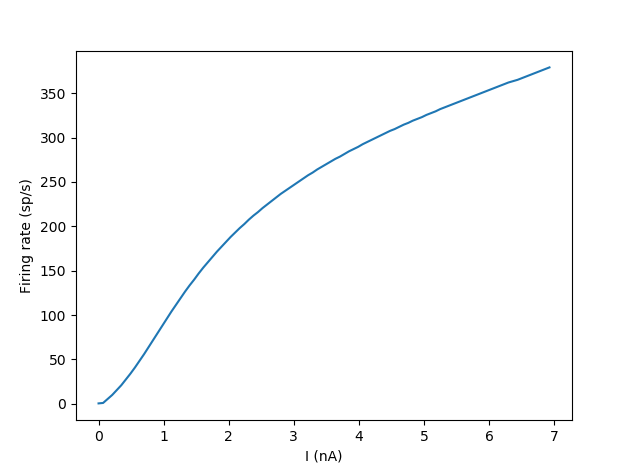
\includegraphics[width=.8\textwidth]{h3_p1.png} %1.png是图片文件的相对路径
  \label{img} %此处的label相当于一个图片的专属标志,目的是方便上下文的引用
  \caption{Result 3.1}
\end{figure}

\newpage
\textbf{Part 4 Linear Integrate and Fire Neuron}
\\

Remove	the	Sodium	and	Potassium	currents	from	the	HH	model in	Problem	1,	
leaving	just	the	leakage current.	Set	EL=-60.0	mV. Set	the	threshold	to	
-40mV.	When	the	potential	hits	threshold,	reset	to	-60	mV	with
$$group	=	NeuronGroup(num_neurons,	eqs,	threshold='v	>	-30*mV',reset='v	=	-
50*mV',$$
$$method='euler')	$$
Compute	the	I	vs	Firing	rate	plot	again	using
$$group.I	=	'(7.0*nA	*	i)	/	num_neurons'$$
Show	an	example	output	from	neuron	75.
 \begin{figure}[H]
  \centering
  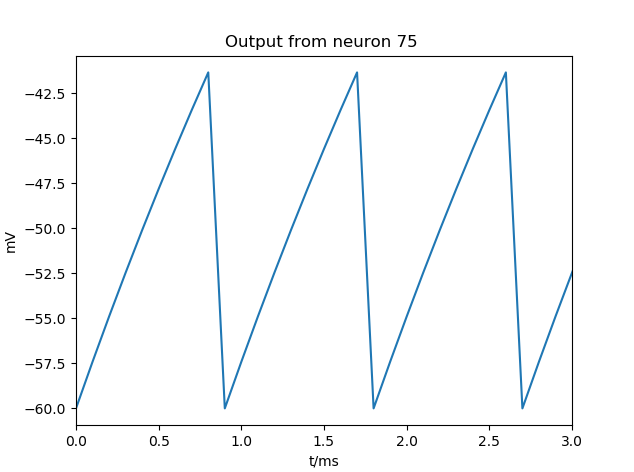
\includegraphics[width=.5\textwidth]{h4_p1_out.png} %1.png是图片文件的相对路径
  \label{img} %此处的label相当于一个图片的专属标志,目的是方便上下文的引用
  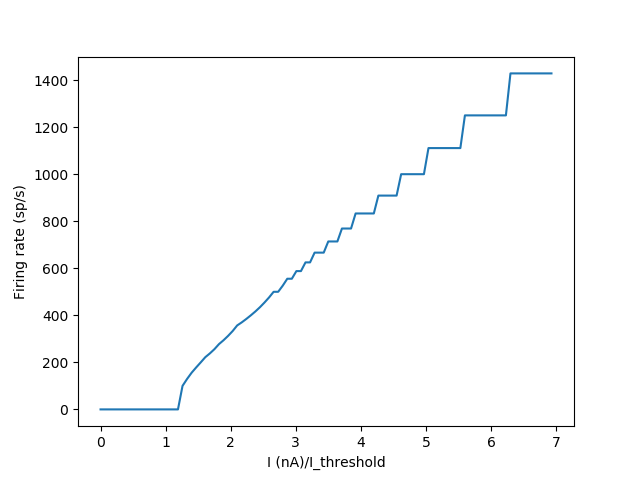
\includegraphics[width=.5\textwidth]{h4_p1_fr.png} %1.png是图片文件的相对路径
  \label{img} %此处的label相当于一个图片的专属标志,目的是方便上下文的引用
  \caption{Result 4.1}
\end{figure}
\newpage
\large \textbf{Appendix}
\\

\normalsize\textbf{Part 1}
\\

\textbf{Problem 1}
\lstset{language=Python}
\begin{lstlisting}
from brian2 import *

num_neurons = 2

# Parameters
area=20000*umetre**2
Cm = 1*ufarad*cm**-2
El = 10.613*mV
EK = -12.0*mV
ENa = 115.0*mV
E_rest = 0*mV

gl = 0.3*(msiemens)/(cm**2)
gNa = 120.0*(msiemens)/(cm**2)
gK = 36.0*(msiemens)/(cm**2)


#The model
eqs_ina = '''
ina=gNa * m**3 * h * (ENa-((v+60*mV))) :  amp/meter**2

dm/dt = alpham * (1-m) - betam * m : 1
dh/dt = alphah * (1-h) - betah * h : 1

alpham = (0.1/mV) * (-(v+60*mV)+25*mV) / (exp((-(v+60*mV)+25*mV) / (10*mV)) - 1) /ms : Hz
betam = 4*exp(-(v+60*mV)/(18*mV))/ms : Hz
alphah = 0.07*exp(-(v+60*mV)/(20*mV))/ms : Hz
betah = 1/(exp((-(v+60*mV)+30*mV) / (10*mV))+1)/ms : Hz
'''

eqs_ik = '''
ik=gK * n**4 * (EK-(v+60*mV)):amp/meter**2

dn/dt = alphan * (1-n) - betan * n : 1

alphan = (0.01/mV) * (-(v+60*mV)+10*mV) / (exp((-(v+60*mV)+10*mV) / (10*mV)) - 1)/ms : Hz
betan = 0.125*exp(-(v+60*mV)/(80*mV))/ms : Hz
'''

eqs_il = '''
il = gl * (El-(v+60*mV)) :amp/meter**2
'''

eqs = '''
dv/dt = (ina+ik+il +I/area)/Cm :  volt
I : amp
'''
eqs += (eqs_ina+eqs_ik+eqs_il)

# Threshold and refractoriness are only used for spike counting
group = NeuronGroup(num_neurons, eqs,
                    threshold='v > -100*mV',
                    refractory='v > -100*mV',
                    method='exponential_euler')
group.v = -60*mV
group.m=0.0529
group.n=0.3177
group.h=0.596

monitor2=StateMonitor(group,'v',record=True)
group.I = 0*nA
run(5.0*ms,report='text')
group.I[0] = 1.50*nA
group.I[1] = 1.90*nA
run(1*ms, report='text')
group.I = 0*nA
run(14.0*ms)


figure(1)
plot(monitor2.t/ms, monitor2.v[0]/mV) #plot the voltage for neuron 0 (index starts at 0)
plot(monitor2.t/ms, monitor2.v[1]/mV) #plot the voltage for neuron 0 (index starts at 0)
# ylim(-20,120) #set axes limits
# xlim(0,20)
xlabel('Time (ms)')
ylabel('Voltage (mV)')
title('Hodgkin-Huxley Action Potential, Rest Potential = 0mV')

#You can dump your results to a file to visualize separately 
savetxt('Vmdata.dat',(monitor2.t/ms, monitor2.v[0]/mV))
#out=np.loadtxt('Vmdata.dat')
#plot(out[0],out[1])
show()
\end{lstlisting}
\newpage

\textbf{Problem 2}
\lstset{language=Python}
\begin{lstlisting}
from brian2 import *

num_neurons = 2
num_E_rest = -60
# Parameters
area=20000*umetre**2
Cm = 1*ufarad*cm**-2
El = -49.387*mV
EK = -72.0*mV
ENa = 55.0*mV
E_rest = -60*mV
duration = 2*second
gl = 0.3*(msiemens)/(cm**2)
gNa = 120.0*(msiemens)/(cm**2)
gK = 36.0*(msiemens)/(cm**2)


#The model
eqs_ina = '''
ina=gNa * m**3 * h * (ENa-(v)) :  amp/meter**2

dm/dt = alpham * (1-m) - betam * m : 1
dh/dt = alphah * (1-h) - betah * h : 1

alpham = (0.1/mV) * (-(v+60*mV)+25*mV) / (exp((-(v+60*mV)+25*mV) / (10*mV)) - 1) /ms : Hz
betam = 4*exp(-(v+60*mV)/(18*mV))/ms : Hz
alphah = 0.07*exp(-(v+60*mV)/(20*mV))/ms : Hz
betah = 1/(exp((-(v+60*mV)+30*mV) / (10*mV))+1)/ms : Hz
'''

eqs_ik = '''
ik=gK * n**4 * (EK-v):amp/meter**2

dn/dt = alphan * (1-n) - betan * n : 1

alphan = (0.01/mV) * (-(v+60*mV)+10*mV) / (exp((-(v+60*mV)+10*mV) / (10*mV)) - 1)/ms : Hz
betan = 0.125*exp(-(v+60*mV)/(80*mV))/ms : Hz
'''

eqs_il = '''
il = gl * (El-v) :amp/meter**2
'''

eqs = '''
dv/dt = (ina+ik+il +I/area)/Cm :  volt
I : amp
'''
eqs += (eqs_ina+eqs_ik+eqs_il)

# Threshold and refractoriness are only used for spike counting
group = NeuronGroup(num_neurons, eqs,
                    threshold='v > -40*mV',
                    refractory='v > -40*mV',
                    method='exponential_euler')
group.v = -60*mV
group.m=0.0529
group.n=0.3177
group.h=0.596

monitor2=StateMonitor(group,'v',record=True)
group.I = 0*nA
run(5.0*ms, report='text')
group.I[0] = 1.50*nA
group.I[1] = 1.90*nA

run(1*ms, report='text')
group.I = 0*nA
run(14.0*ms)

signal = 0
figure(1)
for ii in range(num_neurons):
    plot(monitor2.t / ms, monitor2.v[ii] / mV)  # plot the voltage for neuron 0 (index starts at 0)
    if max(monitor2.v[ii] / mV) > 0 and signal == 0:
        print("The "+ str(ii)+ " neuron is fired, and the amplitude of current is " + str(1.50 + ii * 0.1) + "nA")
        signal = 1
ylim(-90, 50) #set axes limits
# xlim(0, 20)
xlabel('Time (ms)')
ylabel('Voltage (mV)')
legend()
title('Hodgkin-Huxley Action Potential, Rest Potential ='+ str(num_E_rest) + ' mV')

show()
\end{lstlisting}
\newpage

\textbf{Problem 3}
\lstset{language=Python}
\begin{lstlisting}
from brian2 import *

num_neurons = 100
num_E_rest = -60
# Parameters
area=20000*umetre**2
Cm = 1*ufarad*cm**-2
El = -49.387*mV
EK = -72.0*mV
ENa = 55.0*mV
E_rest = -60*mV
duration = 2*second
gl = 0.3*(msiemens)/(cm**2)
gNa = 120.0*(msiemens)/(cm**2)
gK = 36.0*(msiemens)/(cm**2)


#The model
eqs_ina = '''
ina=gNa * m**3 * h * (ENa-(v)) :  amp/meter**2

dm/dt = alpham * (1-m) - betam * m : 1
dh/dt = alphah * (1-h) - betah * h : 1

alpham = (0.1/mV) * (-(v+60*mV)+25*mV) / (exp((-(v+60*mV)+25*mV) / (10*mV)) - 1) /ms : Hz
betam = 4*exp(-(v+60*mV)/(18*mV))/ms : Hz
alphah = 0.07*exp(-(v+60*mV)/(20*mV))/ms : Hz
betah = 1/(exp((-(v+60*mV)+30*mV) / (10*mV))+1)/ms : Hz
'''

eqs_ik = '''
ik=gK * n**4 * (EK-v):amp/meter**2

dn/dt = alphan * (1-n) - betan * n : 1

alphan = (0.01/mV) * (-(v+60*mV)+10*mV) / (exp((-(v+60*mV)+10*mV) / (10*mV)) - 1)/ms : Hz
betan = 0.125*exp(-(v+60*mV)/(80*mV))/ms : Hz
'''

eqs_il = '''
il = gl * (El-v) :amp/meter**2
'''

eqs = '''
dv/dt = (ina+ik+il +I/area)/Cm :  volt
I : amp
'''
eqs += (eqs_ina+eqs_ik+eqs_il)

# Threshold and refractoriness are only used for spike counting
group = NeuronGroup(num_neurons, eqs,
                    threshold='v > -40*mV',
                    refractory='v > -40*mV',
                    method='exponential_euler')
group.v = -60*mV
group.m=0.0529
group.n=0.3177
group.h=0.596

monitor2=StateMonitor(group,'v',record=True)
group.I = 0*nA
run(5.0*ms, report='text')
for i in range(num_neurons):
    group.I[i] = (1.0 + 0.01*i)*nA

# group.I[0] = 1.50*nA
# group.I[1] = 2.50*nA
run(1*ms, report='text')
group.I = 0*nA
run(14.0*ms)

signal = 0
figure(1)
for ii in range(num_neurons):
    plot(monitor2.t / ms, monitor2.v[ii] / mV)  # plot the voltage for neuron 0 (index starts at 0)
    if max(monitor2.v[ii] / mV) > 0 and signal == 0:
        print("The "+ str(ii+1)+ " neuron is fired, and the amplitude of current is " + str(1.0 + ii * 0.01) + "nA")
        signal = 1
# plot(monitor2.t/ms, monitor2.v[0]/mV) #plot the voltage for neuron 0 (index starts at 0)
# plot(monitor2.t/ms, monitor2.v[1]/mV) #plot the voltage for neuron 0 (index starts at 0)
ylim(-90, 50) #set axes limits
# xlim(0, 20)
xlabel('Time (ms)')
ylabel('Voltage (mV)')
legend()
title('Hodgkin-Huxley Action Potential, Rest Potential ='+ str(num_E_rest) + ' mV')

#You can dump your results to a file to visualize separately
# savetxt('Vmdata.dat',(monitor2.t/ms, monitor2.v[0]/mV))
#out=np.loadtxt('Vmdata.dat')
#plot(out[0],out[1])
show()
\end{lstlisting}
\newpage

\textbf{Problem 4}
\lstset{language=Python}
\begin{lstlisting}
from brian2 import *

num_neurons = 100
num_E_rest = -60
# Parameters
area=20000*umetre**2
Cm = 1*ufarad*cm**-2
El = -49.387*mV
EK = -72.0*mV
ENa = 55.0*mV
E_rest = -60*mV
duration = 2*second
gl = 0.3*(msiemens)/(cm**2)
gNa = 120.0*(msiemens)/(cm**2)
gK = 36.0*(msiemens)/(cm**2)


#The model
eqs_ina = '''
ina=gNa * m**3 * h * (ENa-(v)) :  amp/meter**2

dm/dt = alpham * (1-m) - betam * m : 1
dh/dt = alphah * (1-h) - betah * h : 1

alpham = (0.1/mV) * (-(v+60*mV)+25*mV) / (exp((-(v+60*mV)+25*mV) / (10*mV)) - 1) /ms : Hz
betam = 4*exp(-(v+60*mV)/(18*mV))/ms : Hz
alphah = 0.07*exp(-(v+60*mV)/(20*mV))/ms : Hz
betah = 1/(exp((-(v+60*mV)+30*mV) / (10*mV))+1)/ms : Hz
'''

eqs_ik = '''
ik=gK * n**4 * (EK-v):amp/meter**2

dn/dt = alphan * (1-n) - betan * n : 1

alphan = (0.01/mV) * (-(v+60*mV)+10*mV) / (exp((-(v+60*mV)+10*mV) / (10*mV)) - 1)/ms : Hz
betan = 0.125*exp(-(v+60*mV)/(80*mV))/ms : Hz
'''

eqs_il = '''
il = gl * (El-v) :amp/meter**2
'''

eqs = '''
dv/dt = (ina+ik+il +I/area)/Cm :  volt
I : amp
'''
eqs += (eqs_ina+eqs_ik+eqs_il)

# Threshold and refractoriness are only used for spike counting
group = NeuronGroup(num_neurons, eqs,
                    threshold='v > -40*mV',
                    refractory='v > -40*mV',
                    method='exponential_euler')
group.v = -60*mV
group.m=0.0529
group.n=0.3177
group.h=0.596

monitor2=StateMonitor(group,'v',record=True)

group.I = '(7.0*nA * i) / num_neurons'
monitor = SpikeMonitor(group)
run(duration)
print(monitor.count)
figure(1)
plot(group.I/nA, (monitor.count / duration)/Hz)
xlabel('I (nA)')
ylabel('Firing rate (sp/s)')

show()
\end{lstlisting}
\newpage

\normalsize\textbf{Part 2}
\\

\textbf{Problem 1}
\lstset{language=Python}
\begin{lstlisting}
from brian2 import *

num_neurons = 100
duration = 2*second

# Parameters
area = 20000*umetre**2
Cm = 1*ufarad*cm**-2
El = -17.0*mV
EK = -72*mV
ENa = 55.0*mV
EA= -75.0*mV

gl = 0.3*msiemens/cm**2
gNa = 120.0*msiemens/cm**2
gK = 20*msiemens/cm**2
gA = 47.7*msiemens/cm**2

#The model
eqs_ina = '''
ina=gNa * m**3 * h * (ENa-v) :  amp/meter**2
dm/dt = alpham * (1-m) - betam * m : 1
dh/dt = alphah * (1-h) - betah * h : 1
alpham = 0.38/mV*(v+29.7*mV)/(1-exp(-0.1*(v+29.7*mV)/mV ) )/ms : Hz
betam = 15.2*exp(-0.0556*(v+54.7*mV)/mV)/ms : Hz
alphah = 0.266*exp(-0.05*(v+48*mV)/mV)/ms : Hz
betah = 3.8/(1+exp(-0.1*(v+18.*mV)/mV))/ms : Hz
'''




eqs_iA = '''
iA=gA * a**3 * b * (EA-v) :  amp/meter**2
a_inf = (((0.0761*exp(0.0314*(v+94.22*mV)/mV))/(1+exp(0.0346*(v+1.17*mV)/mV)))**(1/3)) : 1
b_inf = ((1/(1+exp(0.0688*(v+53.3*mV)/mV)))**4) : 1
da/dt = (a_inf - a)/tau_a : 1
db/dt = (b_inf - b)/tau_b : 1
tau_a = (0.3632 + (1.158/(1+exp(0.0497*(v+55.96*mV)/mV))))*ms : second
tau_b = (1.24 + (2.678/(1+exp(0.0624*(v+50*mV)/mV))))*ms : second
'''

eqs_ik = '''
ik=gK * n**4 * (EK-v):amp/meter**2
dn/dt = alphan * (1-n) - betan * n : 1
alphan = (0.02*(v+45.7*mV)/mV)/(1-exp(-0.1*(v+45.7*mV)/mV))/ms : Hz
betan = 0.25*exp(-0.0125*(v+55.7*mV)/mV)/ms : Hz
'''

eqs_il = '''
il = gl * (El-v) :amp/meter**2
'''

eqs = '''
dv/dt = (ina+ik+il+iA+I/area)/Cm:  volt
I : amp
'''
eqs += (eqs_ina+eqs_ik+eqs_il+eqs_iA)
# re-run spikes
# Threshold and refractoriness are only used for spike counting

group = NeuronGroup(num_neurons, eqs,
                    threshold='v > -40*mV',
                    refractory='v > -40*mV',
                    method='exponential_euler')
# group.v = -90.0*mV
# # group.m=0.0529
# # group.n=0.3177
# # group.h=0.596
# group.m=0
# group.n=0
# group.h=1
group.v = -89.79961487*mV
group.m=0.00052483
group.n=0.02756506
group.h=0.99865692
group.a = 0.4371503
group.b =0.73184542
group.I = -13.0*nA
monitor2=StateMonitor(group,'v',record=True)
run(50.0*ms)
group.I = '(7.0*nA * i) / num_neurons'

monitor = SpikeMonitor(group)

run(duration)
fig = figure(figsize=(7, 7))

ax4 = fig.add_subplot(224)
plot(monitor2.t/ms, monitor2.v[28]/mV) #plot the voltage for neuron 0 (index starts at 0)
xlim(0, 200)
xlabel('t/ms')
ylabel('mV')

# Threshold and refractoriness are only used for spike counting
group = NeuronGroup(num_neurons, eqs,
                    threshold='v > -40*mV',
                    refractory='v > -40*mV',
                    method='exponential_euler')
group.v = -66.76811498*mV
group.m=0.01287421
group.n=0.67802686
group.h=0.26582129
group.a=0.7364238
group.b=0.03608132
# group.v = -70.0*mV
# group.m=0.0
# group.n=0.7
# group.h=0.5


monitor2=StateMonitor(group, 'v', record=True)

group.I = '(7.0*nA * i) / num_neurons'

monitor = SpikeMonitor(group)

run(duration)

ax1 = fig.add_subplot(221)
plot(group.I/nA/1.615, (monitor.count / duration)/Hz)
xlim(0.9, 1.5)
xticks(arange(0.9, 1.6, 0.1))
ylim(0, 60)
xlabel('I (nA)/I_threshold')
ylabel('Firing rate (sp/s)')
ax2 = fig.add_subplot(222)
plot(monitor2.t/ms, monitor2.v[29]/mV) #plot the voltage for neuron 0 (index starts at 0)
xlim(0, 100)
xlabel('t/ms')
ylabel('mV')


# turned off
gA=  0 *msiemens/cm**2
El = -70*mV
num_neurons = 1000
# Threshold and refractoriness are only used for spike counting
group = NeuronGroup(num_neurons, eqs,
                    threshold='v > -40*mV',
                    refractory='v > -40*mV',
                    method='exponential_euler')
group.v = -68.0*mV
group.m=0.0529
group.n=0.3177
group.h=0.596

monitor2=StateMonitor(group,'v',record=True)

group.I = '(7.0*nA * i) / num_neurons'

monitor = SpikeMonitor(group)

run(duration)
ax3 = fig.add_subplot(223)
plot(group.I/nA/1.54, (monitor.count / duration)/Hz)
xlim(0.9, )
ylim(0, 200)
xlabel('I (nA)/I_threshold')
ylabel('Firing rate (sp/s)')


show()
\end{lstlisting}
\newpage

\normalsize\textbf{Part 3}
\\

\textbf{Problem 1}
\lstset{language=Python}
\begin{lstlisting}
from brian2 import *

num_neurons = 100
duration = 2.0 * second

# Parameters
area = 20000 * umetre ** 2
Cm = (1 * ufarad * cm ** -2)
defaultclock.dt = .02 * ms
div = defaultclock.dt

# The model

ENa = 50.0 * mV
gnabar = 50 * msiemens * cm ** -2
VT1 = -61.5 * mV
VT = -61.5 * mV
EK = -90.0 * mV
gkbar = 4.8 * msiemens * cm ** -2
EKm = -90.0 * mV
gmbar = 0.15* msiemens * cm ** -2
glbar = 0.0205 * msiemens / cm ** 2
El = -70 * mV
tau_max = 1123.5*ms

eqs_na = """
ina = gnabar*m**3*h*(ENa-v) : amp/meter**2
dm/dt  = (am1*(1-m)-bm1*m): 1
dh/dt  = (ah1*(1-h)-bh1*h): 1
am1=0.32*(13-(vu-VT/mV))/(exp((13-(vu-VT/mV))/4.0)-1.0)/ms: Hz
bm1=(0.28*((vu-VT/mV)-40)/(exp(((vu-VT/mV)-40)/5.0)-1.0))/ms: Hz
ah1 = 0.128*exp(-(vu-17-VT/mV)/18)/ms: Hz
bh1 = 4/(1+exp(-(vu-40-VT/mV)/5))/ms: Hz
"""

# IM channel () non-inactivating
eqs_m = """
im = gmbar*c*(EKm-v) : amp/meter**2
dc/dt = ((cv - c)/tau_c) : 1
cv = 1/(1+exp(-(v/mV+35)/10)) : 1
tau_c = (tau_max/(3.3*exp(((v+35*mV)/20)/mV)+exp((-(v+35*mV)/20)/mV))) : second
"""

# Delayed Rectifier K channel
eqs_k = """
ik = gkbar*b**4*(EK-v): amp/meter**2
db/dt  = (ab*(1-b)-bb*b): 1
ab=0.032*(vu-15-VT1/mV)/(1.0 - exp(-(vu-15-VT1/mV)/5.0))/ms:Hz
bb=0.5*exp(-(vu-10-VT1/mV)/40)/ms : Hz

"""

# Leak
eqs_leak = """
il = glbar*(El-v) : amp/meter**2
"""

eqs = """
dv/dt = (il + ik+ +ina+ im + I/area)/Cm : volt
vu = v/mV : 1  # unitless v 
I: amp
"""
eqs += eqs_leak + eqs_k + eqs_na + eqs_m

# Threshold and refractoriness are only used for spike counting
P1 = NeuronGroup(num_neurons, eqs, clock=Clock(defaultclock.dt),
                 threshold='v > -40*mV', refractory='v > -40*mV', method='euler')

P1.I	='(7.0*nA*i)/num_neurons'

monitor = SpikeMonitor(P1)
monitor2 = StateMonitor(P1, ('v'), record=True)
net = Network(P1, monitor, monitor2)
net.run(duration)

figure(1)
plot(P1.I / nA, monitor.count / duration)
xlabel('I (nA)')
ylabel('Firing rate (sp/s)')
show()
\end{lstlisting}
\newpage

\normalsize\textbf{Part 4}
\\

\textbf{Problem 1}
\lstset{language=Python}
\begin{lstlisting}
from brian2 import *

num_neurons = 100
duration = 2000*ms
# Parameters
area=20000*umetre**2
Cm = 1*ufarad*cm**-2
El = -60*mV
EK = -72.0*mV
ENa = 55.0*mV
E_rest = -60*mV

gl = 0.3*(msiemens)/(cm**2)
gNa = 120.0*(msiemens)/(cm**2)
gK = 36.0*(msiemens)/(cm**2)


#The model
eqs_il = '''
il = gl * (El-v) :amp/meter**2
'''

eqs = '''
dv/dt = (il +I/area)/Cm :  volt
I : amp
'''
eqs += (eqs_il)

# Threshold and refractoriness are only used for spike counting
group = NeuronGroup(num_neurons, eqs,
                    threshold='v > -40*mV',
                    reset='v=-60*mV',
                    method='euler')
group.v = -60*mV
monitor2=StateMonitor(group,'v',record=True)
group.I = '(7.0*nA * i) / num_neurons'

monitor = SpikeMonitor(group)

run(duration)
figure(1)
plot(monitor2.t/ms, monitor2.v[74]/mV) #plot the voltage for neuron 0 (index starts at 0)
xlim(0, 3)
xlabel('t/ms')
ylabel('mV')
title('Output from neuron 75 ')
figure(2)
plot(group.I/nA, (monitor.count / duration)/Hz)
xlabel('I (nA)/I_threshold')
ylabel('Firing rate (sp/s)')
show()
\end{lstlisting}
\newpage

\end{document}